\pagebreak
Block name: vmm12$\times$1\_wowta

Number of inputs: 12

Number of outputs: 1

Parameter list: Input\_Dimensions, Weight\_Matrix, Offset\_bias

Block description: 
This is a Vector Matrix Multiplie circuit built using Floating Gate (FG) pFET transistors. There are 12 input FG pFET transistors
and an offset FG transistor. Input\_Dimensions has row and column depending on inputs for your VMM one can have minimum of 1 input
to maximum of 12 inputs. Output columns can be as many allowed by FPAA. Each VMM block will sit in a different CAB. The inputs and
outputs are vectorized.

\begin{figure}[H]  % jpg, png, or pdf
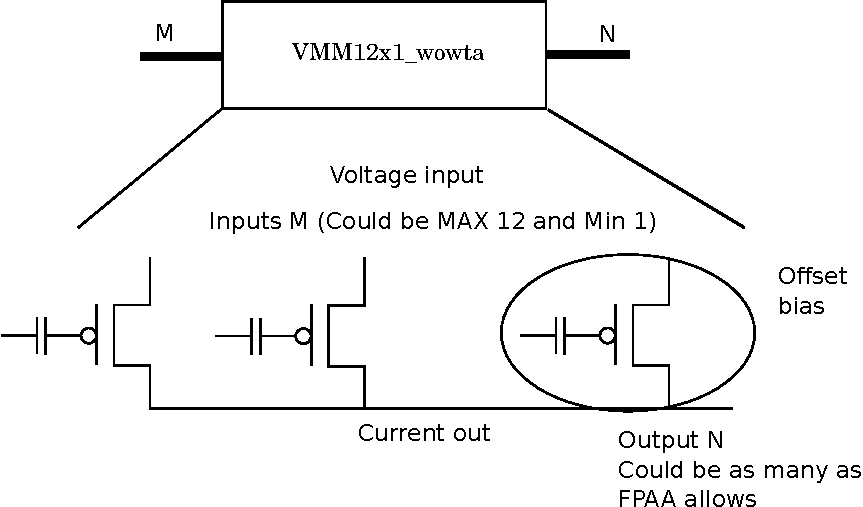
\includegraphics[width=300pt]{$FPAAHOME/rasp30/sci2blif/documentation/blocks_latex/figures/vmm12x1_wowta.pdf}
\end{figure}

